\chapter{System Architecture}

\section{Platform and Technologies Used}
\subsection{Application Server}
\begin{itemize}
\item \textbf{Framework : Ruby On Rails}\\
Ruby on Rails is a web application framework written in Ruby under the MIT License. Rails is a model–view–controller (MVC) framework, providing default structures for a database, a web service, and web pages. The complete framework can be easily setup on system using the following links \cite{Setup43:online} \cite{RVM:R7:online}.

\textbf{Ruby version} : ruby 2.3.0p0 (2015-12-25 revision 53290) [x86\_64-linux] \\
\textbf{Rails version} : Rails 4.2.6

\item \textbf{Network Library} \\
\textbf{RestClient} : A simple HTTP and REST client for Ruby, inspired by the Sinatra microframework style of specifying actions: get, put, post, delete \cite{GitHu91:online}.\\
\textbf{Net::HTTP} : A rich library which can be used to build HTTP user-agents. It is designed to work closely with URI::HTTP\#host, URI::HTTP\#port and URI::HTTP\#request\_uri  \cite{Class28:online}.
\item \textbf{Database} : MySQL Server \\ 
\textbf{MySQL version} : mysql  Ver 14.14 Distrib 5.5.49, for debian-linux-gnu (x86\_64)
\item \textbf{Web Server} :  Puma\\
Puma is a library that provides a very fast and concurrent HTTP 1.1 server for Ruby web applications. It handles multi threading by running multiple worker threads. The number of the threads running at an instant can be altered as per the load on the system \cite{AMode24:online}.\\
Puma version : puma version 3.4.0

\item \textbf{Push Notifications} : Google Cloud Messaging (GCM) Server
\end{itemize}


\subsection{Android Application}

\begin{itemize}
\item \textbf{Framework : Android Studio} \\
Android Studio provides the fastest tools for building apps on every type of Android device. Android Studio is freely available under the Apache License 2.0.

\textbf{Android Studio version} : Version of Android Studio 1.5.0 is used to build the application \cite{Intro42:online}.

\item \textbf{Network Library} \\
Volley library makes executing asynchronous network calls, loading multiple images in the background, and response caching simpler. Android uses volley libraries for asynchronous task communication to the app server \cite{Andro34:online}

\item \textbf{Database} : SQLite \\
Android uses SQLite Database for storing information on phone.

\item \textbf{Android Software Development Kit (SDK)}\\
Minimum SDK build tool and Platform tool with APIs level 21 or above is required to support the working of various libraries on android phones.

\item \textbf{Receive Notifications} : Google Cloud Messaging (GCM) Client
\end{itemize}

\pagebreak
\section{System Flow}

Following Diagram depicts the entire System Flow.\\ \\ \\
\begin{figure}[H]
    \centering
	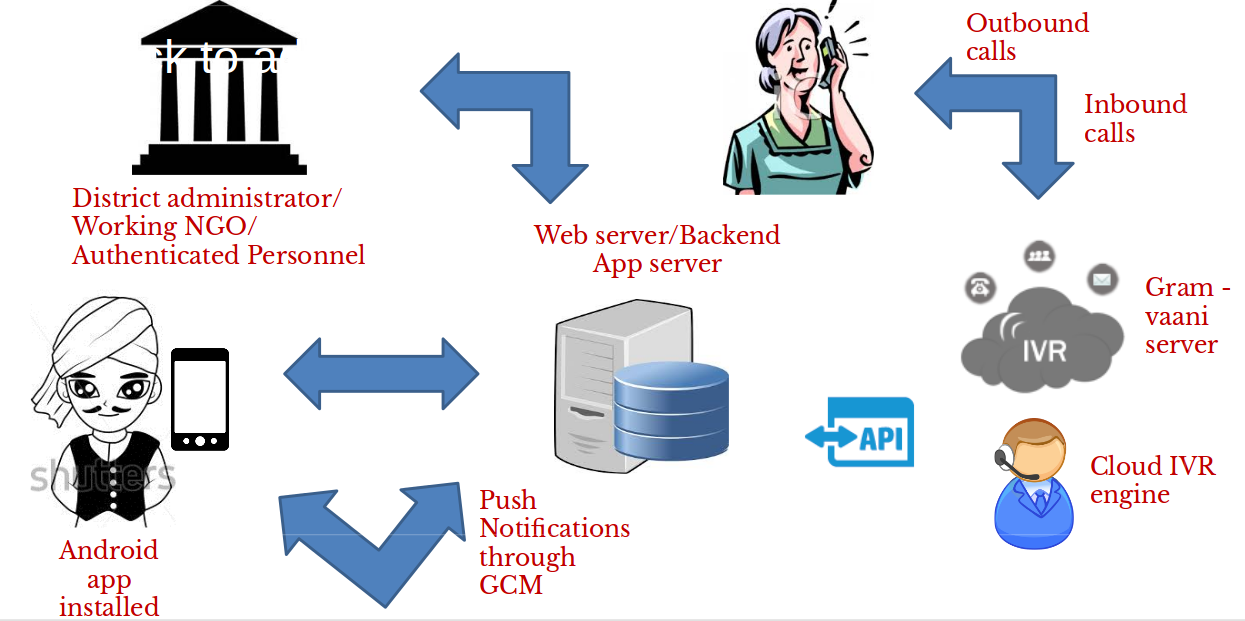
\includegraphics[width=0.8\textwidth]{Sysflow.png}
    \caption{System Flow}
    \label{fig:System Flow}
\end{figure}

\section{Use Case Diagram}
\begin{figure}[H]
    \centering
	\includegraphics[width=0.8\textwidth]{UseCaseDiagram.png}
    \caption{Use Case Diagram of Application User}
    \label{fig:Use Case Diagram of Application User}
\end{figure}

\pagebreak
\section{Entity Relationship Diagram}

Following Diagram depicts the entire database schema design.
\begin{figure}[H]
    \centering
	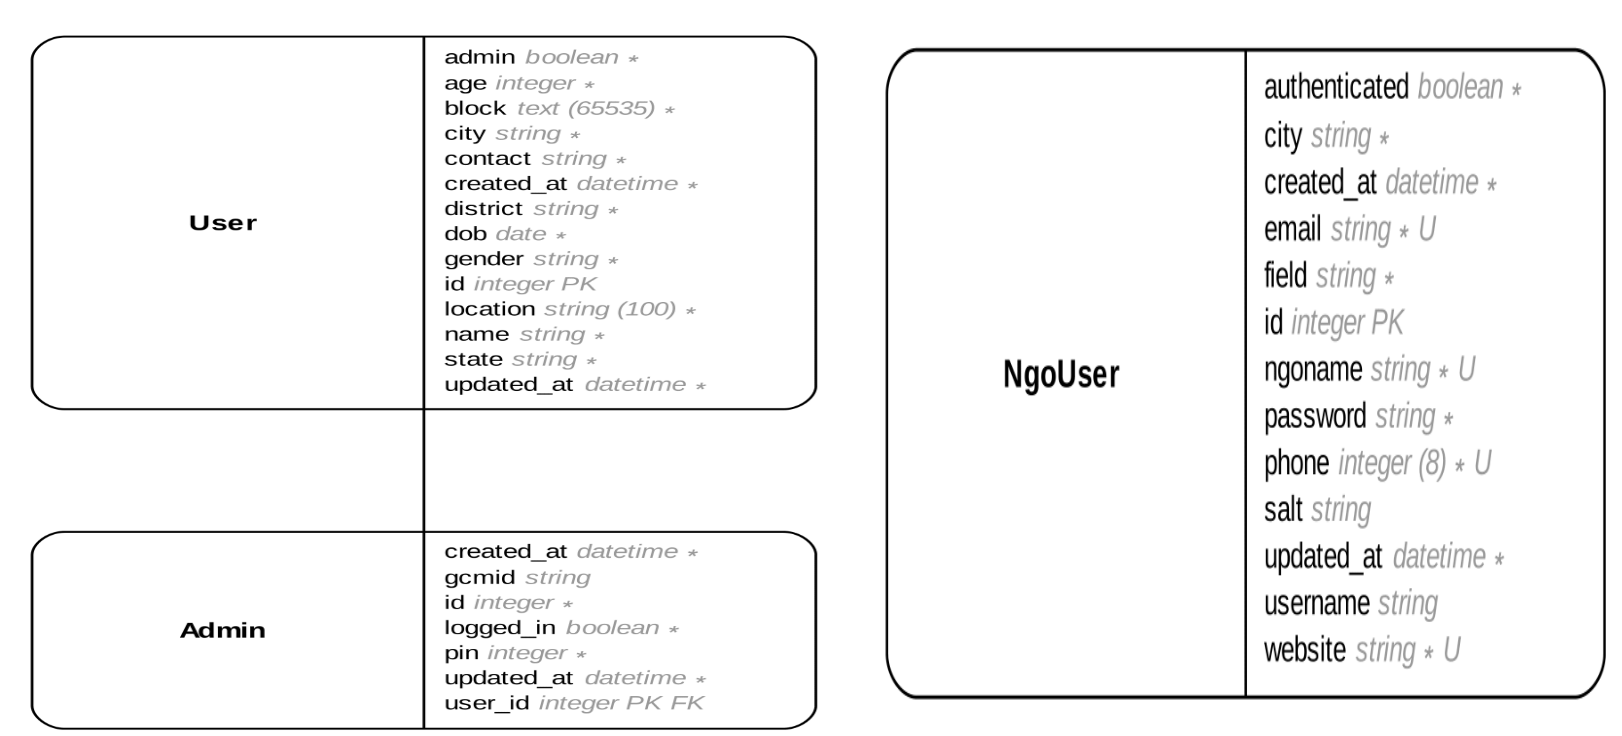
\includegraphics[width=1\textwidth,height=7cm]{erd1.png}
    %\caption{Entity Relationship diagram}
    \label{fig:erd1}
\end{figure}
\begin{figure}[H]
    \centering
	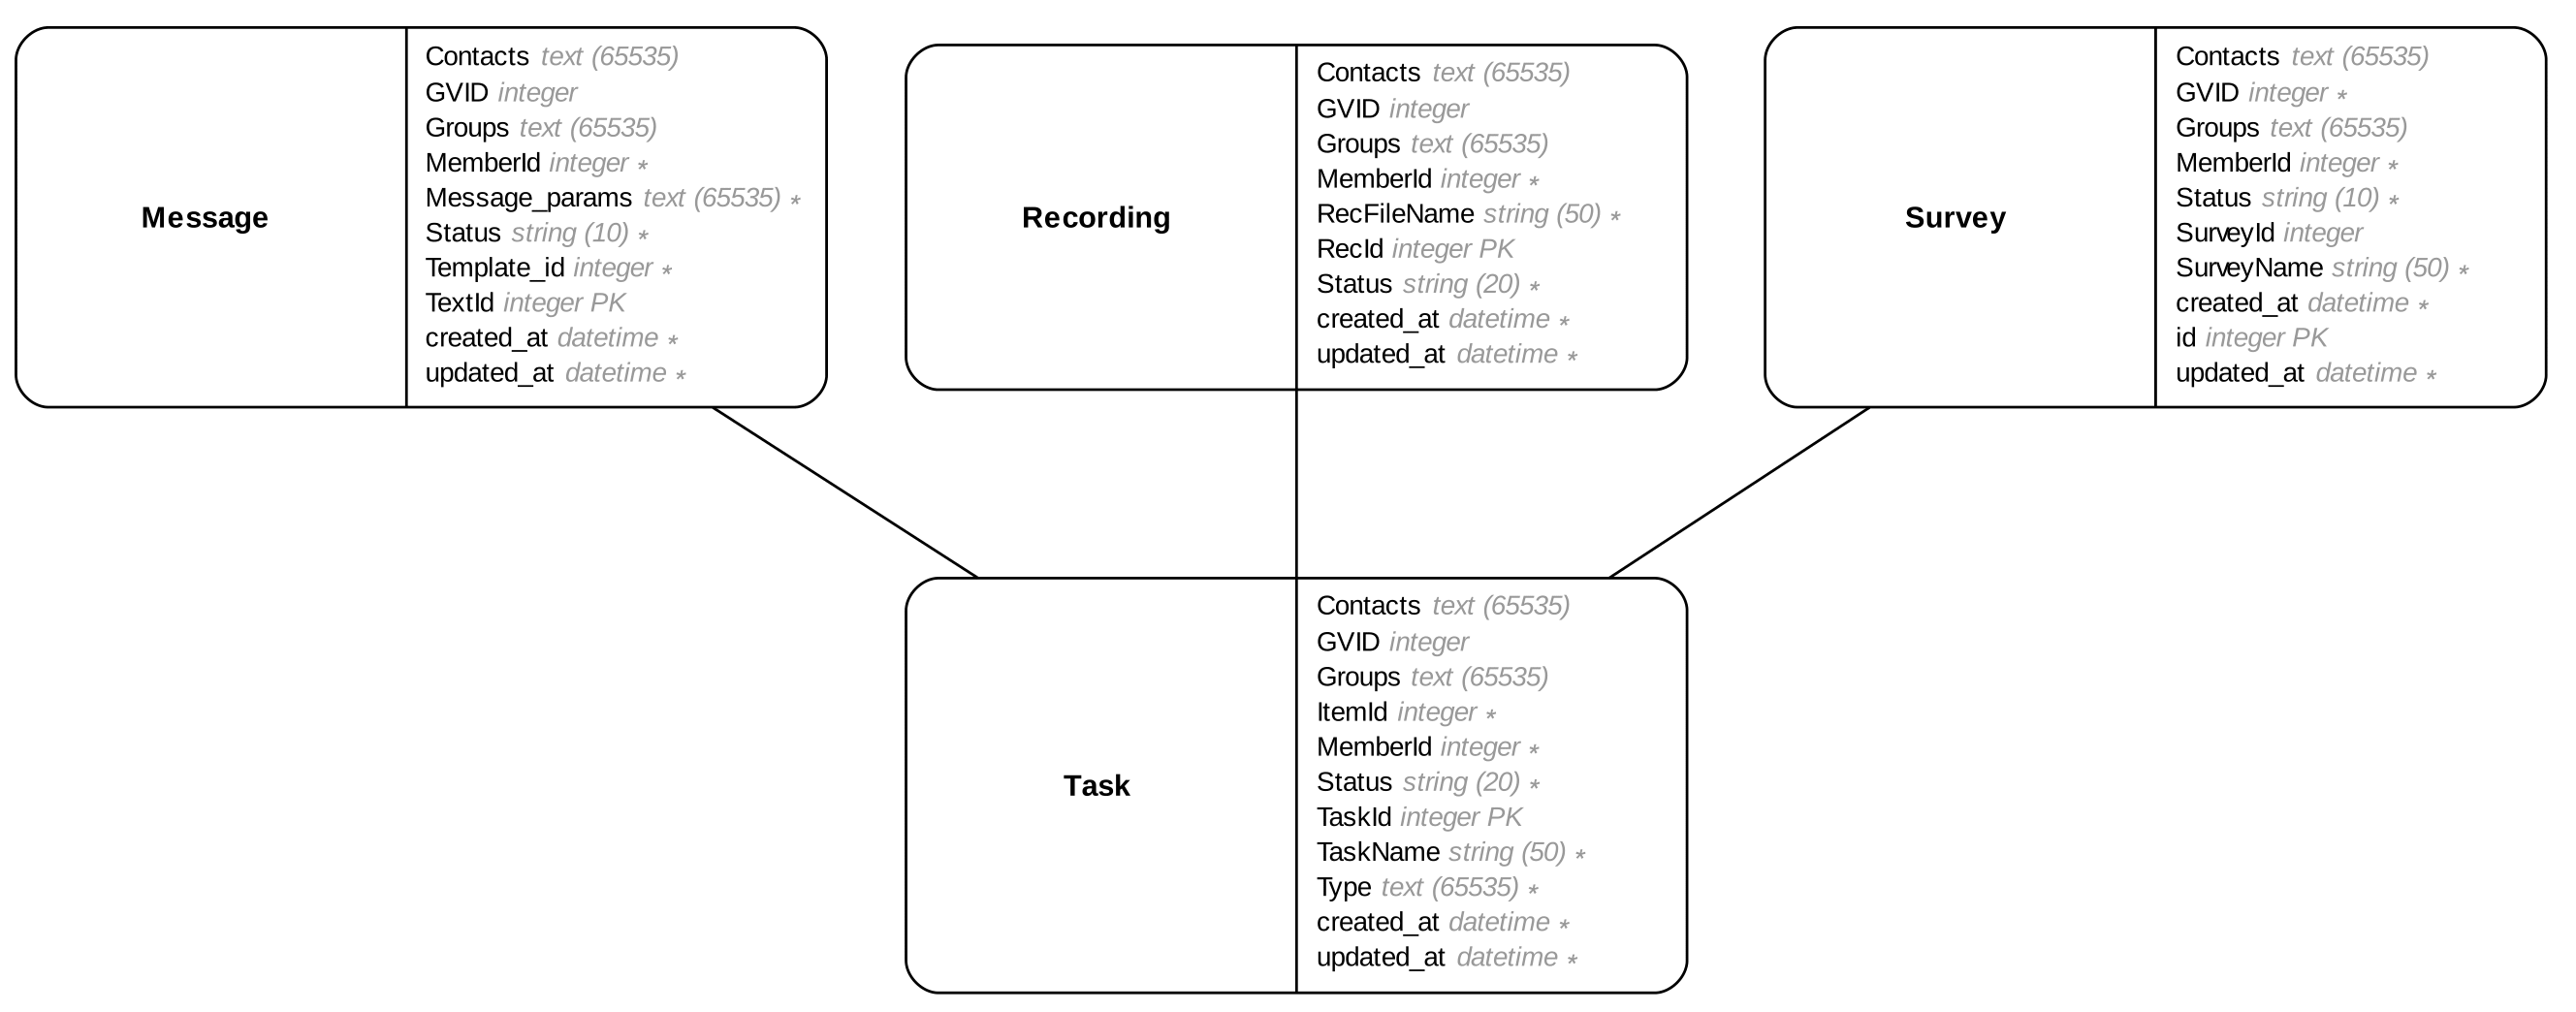
\includegraphics[width=1\textwidth,height=9cm]{erd2.png}
    \caption{Entity Relationship diagram}
    \label{fig:erd2}
\end{figure}
\section{Information flow}
Mobile Application is designed for the volunteers of the village. Along with, a portal is designed for the  NGOs/ Block or district officials for sending alerts to the volunteers of the community. Some volunteers from the community ( For instance, panchayat members, School teachers) will be chosen by the functioning NGO or block/ district administrator under which the community/ village falls. NGOs/ Block or district officials will give authorization to the selected volunteers from that community by registering them through the portal. After authorization, volunteers will be given an Android phone installed with the local governance application "Gologo". Credentials of volunteers will be authenticated on first time login in the application. After successful one time login, volunteers aid their local community people by exploring the app functionalities. Portal will be used to send survey alerts to the volunteers. Volunteers will receive alerts  on their mobile phones to further disperse it to the target people. Through this way, information will flow by the people and  among the people via various functionalities.

%Following Diagram depicts the flow of information through \hyperref[itm:launchsur]{Launch Survey Use Case} whcih is explained later.

%\begin{figure}[H]
 %   \centering
	%\includegraphics[width=0.9\textwidth]%{launchsurvey1.png}
  %  \caption{Launch Survey Use Case}
 %   \label{fig:Launch Survey Use Case}
%\end{figure}
%